\subsection{Magnetometry Experiments on Vapor Cells}
In this experiment, the goal was to demonstrate the
capacity of vapor cells to serve as precise magnetometers in a
laboratory. \\\\ As described in \cite{lucivero2022, tierney2019}, 
when circularly 
polarized light interacts with alkali atoms 
(such as Rubidium or Cesium), it \textit{transfers}
some of its angular momentum into the gas. This effectively generates a
non-zero electron spin polarization state inside the vapor cell.
\\\\
In the presence of an external magnetic field $\vec{B}$, the atomic spins 
undergo Larmor precession at the frequency:
\begin{equation}
    \omega_L = \gamma B
\end{equation}
where $\gamma$ is the gyromagnetic ratio. This precession modulates the projection 
of the atomic spin along the probe beam direction, causing periodic variations 
in the optical absorption and thus in the transmitted light intensity detected 
by the photodiode. When a linear magnetic field ramp --- like $B(t) = B_0 + \alpha t$---
is applied across the vapor cell, the transmitted light intensity exhibits a 
Lorentzian resonance peak centered at $B = 0$. This phenomenon, known
as \textit{Hanle resonance}, arises from the 
following mechanism:
\\\\
For $B \neq 0$, the Zeeman sublevels $(m_F = -F, -F+1, \ldots, +F)$ are 
non-degenerate and precess at different rates, leading to dephasing of the 
atomic coherences. This dephasing destroys the spin polarization created by 
optical pumping, resulting in increased absorption and reduced transmission.
\\\\
At $B = 0$, all Zeeman sublevels become degenerate, eliminating the 
precession-induced dephasing. The atomic coherences remain phase-locked, 
maintaining maximal spin polarization in the direction of the pump beam. 
Atoms in this polarized state exhibit reduced absorption for the circularly 
polarized probe light, producing a transmission maximum.
\\\\ By analyzing the Lorentzian profile, properties of the vapor cell,
such as the coherence lifetime ($\tau$), can be determined. The relationship
between the Lorentzian full width half maximum (FWHM) and $\tau$ is given by:
\begin{equation}
    \Delta B_{FWHM} \sim \frac{1}{\gamma \tau}
\end{equation}

\subsubsection{Experimental Setup}
A \textbf{BRAND AND MODEL} vapor cell was introduced inside
a \textbf{BRAND AND MODEL} magnetic shield, to isolate it from 
background noise (e.g. Earth's magnetic field). A \SI{895}{\nano\meter} laser
is directed into the vapor cell. To control the
power of the incoming light, a half waveplate (HWP) and a polarizing beam 
splitter (PBS) was employed. Just before entering the magnetic shield,
a quarter wave plate (QWP) is placed to generate a circularly polarized beam.
Inside the magnetic shield, coils are used to generate 
an alternating magnetic field in a ramp ($B_x = \alpha t - B_0$)
along the beam axis (X axis). As explaned before, this time-dependent field generates
a time-dependent absorption profile, which is detected in a photodetector placed outside 
the magnetic cavity, connected to a lock-in amplifier. In order to correct background noise, 
DC fields are employed along the Z and Y axis. An illustration of this setup is
displayed in Figure \ref{fig:magnetic_setup}
\begin{figure}
    \centering
    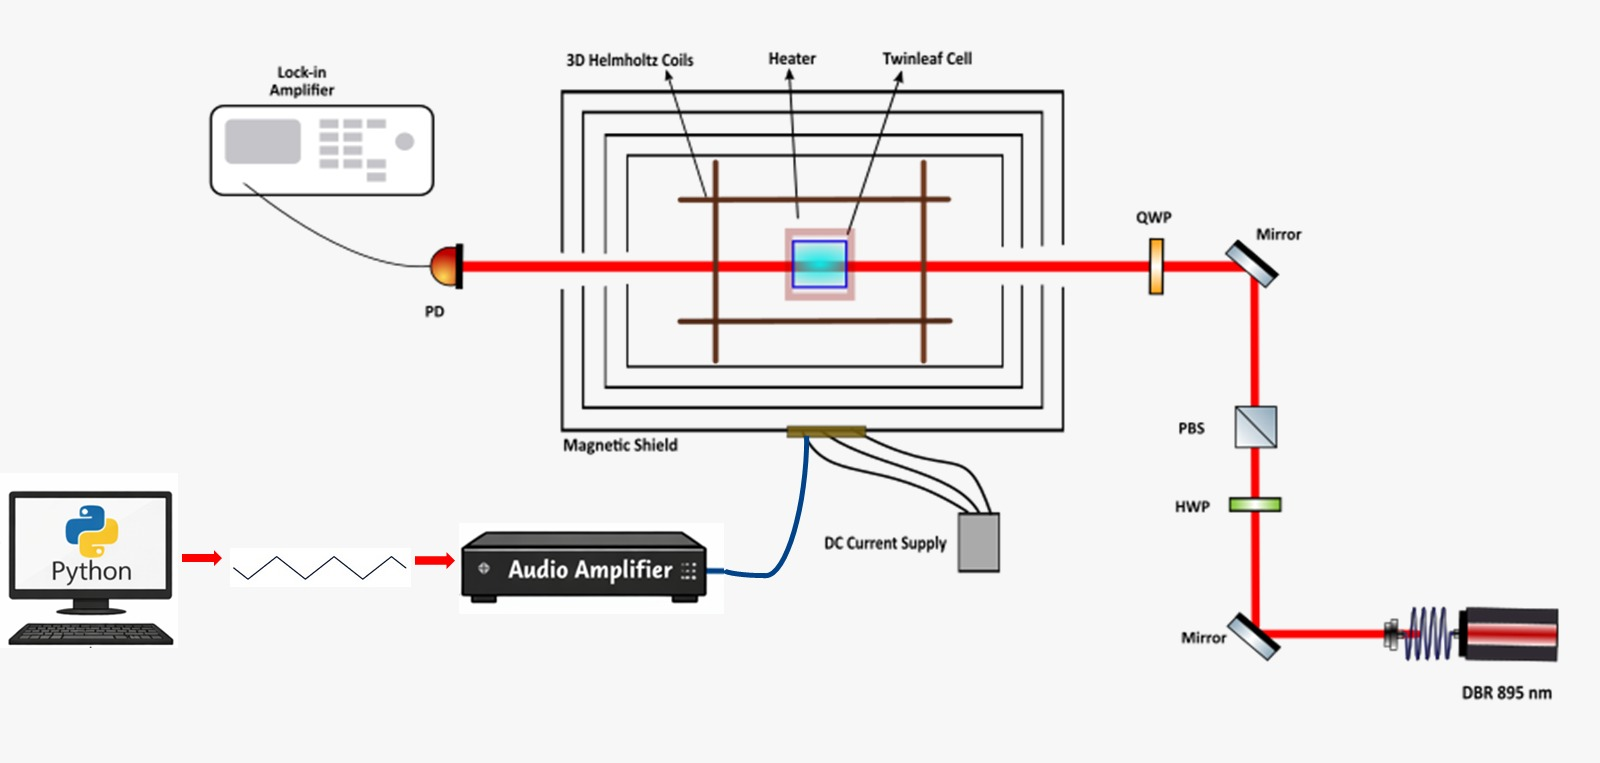
\includegraphics[width=\textwidth]{Images/magnetic_setup.jpg}
    \caption{Experimental setup used to detect Handle resonance}
    \label{fig:magnetic_setup}
\end{figure}

\subsubsection{Results and analysis}
Measurements were made using many different DC field configurations in order to
study the effects on Lorentzian height, width and noise. Figures \ref{fig:magnetic_exp_Zvar}
and \ref{fig:magnetic_exp_Yvar} compare Lorentzian profiles obtained for different DC field
configurations.


